% Options for packages loaded elsewhere
\PassOptionsToPackage{unicode}{hyperref}
\PassOptionsToPackage{hyphens}{url}
\PassOptionsToPackage{dvipsnames,svgnames,x11names}{xcolor}
%
\documentclass[
  letterpaper,
  DIV=11,
  numbers=noendperiod]{scrreprt}

\usepackage{amsmath,amssymb}
\usepackage{iftex}
\ifPDFTeX
  \usepackage[T1]{fontenc}
  \usepackage[utf8]{inputenc}
  \usepackage{textcomp} % provide euro and other symbols
\else % if luatex or xetex
  \usepackage{unicode-math}
  \defaultfontfeatures{Scale=MatchLowercase}
  \defaultfontfeatures[\rmfamily]{Ligatures=TeX,Scale=1}
\fi
\usepackage{lmodern}
\ifPDFTeX\else  
    % xetex/luatex font selection
\fi
% Use upquote if available, for straight quotes in verbatim environments
\IfFileExists{upquote.sty}{\usepackage{upquote}}{}
\IfFileExists{microtype.sty}{% use microtype if available
  \usepackage[]{microtype}
  \UseMicrotypeSet[protrusion]{basicmath} % disable protrusion for tt fonts
}{}
\makeatletter
\@ifundefined{KOMAClassName}{% if non-KOMA class
  \IfFileExists{parskip.sty}{%
    \usepackage{parskip}
  }{% else
    \setlength{\parindent}{0pt}
    \setlength{\parskip}{6pt plus 2pt minus 1pt}}
}{% if KOMA class
  \KOMAoptions{parskip=half}}
\makeatother
\usepackage{xcolor}
\setlength{\emergencystretch}{3em} % prevent overfull lines
\setcounter{secnumdepth}{5}
% Make \paragraph and \subparagraph free-standing
\ifx\paragraph\undefined\else
  \let\oldparagraph\paragraph
  \renewcommand{\paragraph}[1]{\oldparagraph{#1}\mbox{}}
\fi
\ifx\subparagraph\undefined\else
  \let\oldsubparagraph\subparagraph
  \renewcommand{\subparagraph}[1]{\oldsubparagraph{#1}\mbox{}}
\fi


\providecommand{\tightlist}{%
  \setlength{\itemsep}{0pt}\setlength{\parskip}{0pt}}\usepackage{longtable,booktabs,array}
\usepackage{calc} % for calculating minipage widths
% Correct order of tables after \paragraph or \subparagraph
\usepackage{etoolbox}
\makeatletter
\patchcmd\longtable{\par}{\if@noskipsec\mbox{}\fi\par}{}{}
\makeatother
% Allow footnotes in longtable head/foot
\IfFileExists{footnotehyper.sty}{\usepackage{footnotehyper}}{\usepackage{footnote}}
\makesavenoteenv{longtable}
\usepackage{graphicx}
\makeatletter
\def\maxwidth{\ifdim\Gin@nat@width>\linewidth\linewidth\else\Gin@nat@width\fi}
\def\maxheight{\ifdim\Gin@nat@height>\textheight\textheight\else\Gin@nat@height\fi}
\makeatother
% Scale images if necessary, so that they will not overflow the page
% margins by default, and it is still possible to overwrite the defaults
% using explicit options in \includegraphics[width, height, ...]{}
\setkeys{Gin}{width=\maxwidth,height=\maxheight,keepaspectratio}
% Set default figure placement to htbp
\makeatletter
\def\fps@figure{htbp}
\makeatother
% definitions for citeproc citations
\NewDocumentCommand\citeproctext{}{}
\NewDocumentCommand\citeproc{mm}{%
  \begingroup\def\citeproctext{#2}\cite{#1}\endgroup}
\makeatletter
 % allow citations to break across lines
 \let\@cite@ofmt\@firstofone
 % avoid brackets around text for \cite:
 \def\@biblabel#1{}
 \def\@cite#1#2{{#1\if@tempswa , #2\fi}}
\makeatother
\newlength{\cslhangindent}
\setlength{\cslhangindent}{1.5em}
\newlength{\csllabelwidth}
\setlength{\csllabelwidth}{3em}
\newenvironment{CSLReferences}[2] % #1 hanging-indent, #2 entry-spacing
 {\begin{list}{}{%
  \setlength{\itemindent}{0pt}
  \setlength{\leftmargin}{0pt}
  \setlength{\parsep}{0pt}
  % turn on hanging indent if param 1 is 1
  \ifodd #1
   \setlength{\leftmargin}{\cslhangindent}
   \setlength{\itemindent}{-1\cslhangindent}
  \fi
  % set entry spacing
  \setlength{\itemsep}{#2\baselineskip}}}
 {\end{list}}
\usepackage{calc}
\newcommand{\CSLBlock}[1]{\hfill\break\parbox[t]{\linewidth}{\strut\ignorespaces#1\strut}}
\newcommand{\CSLLeftMargin}[1]{\parbox[t]{\csllabelwidth}{\strut#1\strut}}
\newcommand{\CSLRightInline}[1]{\parbox[t]{\linewidth - \csllabelwidth}{\strut#1\strut}}
\newcommand{\CSLIndent}[1]{\hspace{\cslhangindent}#1}

\usepackage{fvextra}
\DefineVerbatimEnvironment{Highlighting}{Verbatim}{breaklines,commandchars=\\\{\}}
\DefineVerbatimEnvironment{OutputCode}{Verbatim}{breaklines,commandchars=\\\{\}}
\KOMAoption{captions}{tableheading}
\makeatletter
\@ifpackageloaded{tcolorbox}{}{\usepackage[skins,breakable]{tcolorbox}}
\@ifpackageloaded{fontawesome5}{}{\usepackage{fontawesome5}}
\definecolor{quarto-callout-color}{HTML}{909090}
\definecolor{quarto-callout-note-color}{HTML}{0758E5}
\definecolor{quarto-callout-important-color}{HTML}{CC1914}
\definecolor{quarto-callout-warning-color}{HTML}{EB9113}
\definecolor{quarto-callout-tip-color}{HTML}{00A047}
\definecolor{quarto-callout-caution-color}{HTML}{FC5300}
\definecolor{quarto-callout-color-frame}{HTML}{acacac}
\definecolor{quarto-callout-note-color-frame}{HTML}{4582ec}
\definecolor{quarto-callout-important-color-frame}{HTML}{d9534f}
\definecolor{quarto-callout-warning-color-frame}{HTML}{f0ad4e}
\definecolor{quarto-callout-tip-color-frame}{HTML}{02b875}
\definecolor{quarto-callout-caution-color-frame}{HTML}{fd7e14}
\makeatother
\makeatletter
\@ifpackageloaded{bookmark}{}{\usepackage{bookmark}}
\makeatother
\makeatletter
\@ifpackageloaded{caption}{}{\usepackage{caption}}
\AtBeginDocument{%
\ifdefined\contentsname
  \renewcommand*\contentsname{Table of contents}
\else
  \newcommand\contentsname{Table of contents}
\fi
\ifdefined\listfigurename
  \renewcommand*\listfigurename{List of Figures}
\else
  \newcommand\listfigurename{List of Figures}
\fi
\ifdefined\listtablename
  \renewcommand*\listtablename{List of Tables}
\else
  \newcommand\listtablename{List of Tables}
\fi
\ifdefined\figurename
  \renewcommand*\figurename{Figure}
\else
  \newcommand\figurename{Figure}
\fi
\ifdefined\tablename
  \renewcommand*\tablename{Table}
\else
  \newcommand\tablename{Table}
\fi
}
\@ifpackageloaded{float}{}{\usepackage{float}}
\floatstyle{ruled}
\@ifundefined{c@chapter}{\newfloat{codelisting}{h}{lop}}{\newfloat{codelisting}{h}{lop}[chapter]}
\floatname{codelisting}{Listing}
\newcommand*\listoflistings{\listof{codelisting}{List of Listings}}
\makeatother
\makeatletter
\makeatother
\makeatletter
\@ifpackageloaded{caption}{}{\usepackage{caption}}
\@ifpackageloaded{subcaption}{}{\usepackage{subcaption}}
\makeatother
\ifLuaTeX
  \usepackage{selnolig}  % disable illegal ligatures
\fi
\usepackage{bookmark}

\IfFileExists{xurl.sty}{\usepackage{xurl}}{} % add URL line breaks if available
\urlstyle{same} % disable monospaced font for URLs
\hypersetup{
  pdftitle={Data Literacy for the Language Sciences},
  pdfauthor={Elen Le Foll},
  colorlinks=true,
  linkcolor={blue},
  filecolor={Maroon},
  citecolor={Blue},
  urlcolor={Blue},
  pdfcreator={LaTeX via pandoc}}

\title{Data Literacy for the Language Sciences}
\usepackage{etoolbox}
\makeatletter
\providecommand{\subtitle}[1]{% add subtitle to \maketitle
  \apptocmd{\@title}{\par {\large #1 \par}}{}{}
}
\makeatother
\subtitle{A very gentle introduction to statistics and data
visualisation in R}
\author{Elen Le Foll}
\date{2024-04-17}

\begin{document}
\maketitle

\renewcommand*\contentsname{Table of contents}
{
\hypersetup{linkcolor=}
\setcounter{tocdepth}{2}
\tableofcontents
}
\bookmarksetup{startatroot}

\chapter*{Preface}\label{preface}
\addcontentsline{toc}{chapter}{Preface}

\markboth{Preface}{Preface}

\begin{tcolorbox}[enhanced jigsaw, colbacktitle=quarto-callout-warning-color!10!white, rightrule=.15mm, breakable, toprule=.15mm, toptitle=1mm, colframe=quarto-callout-warning-color-frame, bottomrule=.15mm, coltitle=black, opacityback=0, titlerule=0mm, opacitybacktitle=0.6, title=\textcolor{quarto-callout-warning-color}{\faExclamationTriangle}\hspace{0.5em}{Warning}, left=2mm, arc=.35mm, leftrule=.75mm, bottomtitle=1mm, colback=white]

This textbook draft is very much \textbf{work in progress}. I intend to
progressively add to it over the course of the summer semester 2024.

This first draft is intended as complementary materials to my summer
semester M.A.~class: ``More than counting words: Introduction to
statistics and data visualisation for linguists'' taught at the
University of Cologne.

Student feedback on this first draft is very welcome!

\end{tcolorbox}

\section*{Who is this book for?}\label{who-is-this-book-for}
\addcontentsline{toc}{section}{Who is this book for?}

\markright{Who is this book for?}

This textbook is intended as a very gentle introduction to basic
principles of data management, statistics, and data visualisation using
the programming language and environment `R`. The target audience are
students and researchers in the language sciences, including (applied)
linguistics, language teaching, and language education research. The
rationale for this textbook is based on my personal observations, in
teaching and consulting both students and researcher colleagues, that
many so-called `introductory' textbooks assume previous knowledge and
skills that all have or go through contents at too fast a pace for many
humanities scholars who often come with little to no experience with
programming and/or statistics.

The aim of this textbook is by no means to replace any of the brilliant
existing textbooks aimed at imparting statistical literacy for
linguistics research, but rather to provide a stepping stone towards
being able to make the most of these wonderful existing resources. A
(work-in-progress) list of next-step resources is included in
\href{https://elenlefoll.github.io/RstatsTextbook/FurtherResources.html}{Appendix
A}.

\begin{figure}[H]

{\centering 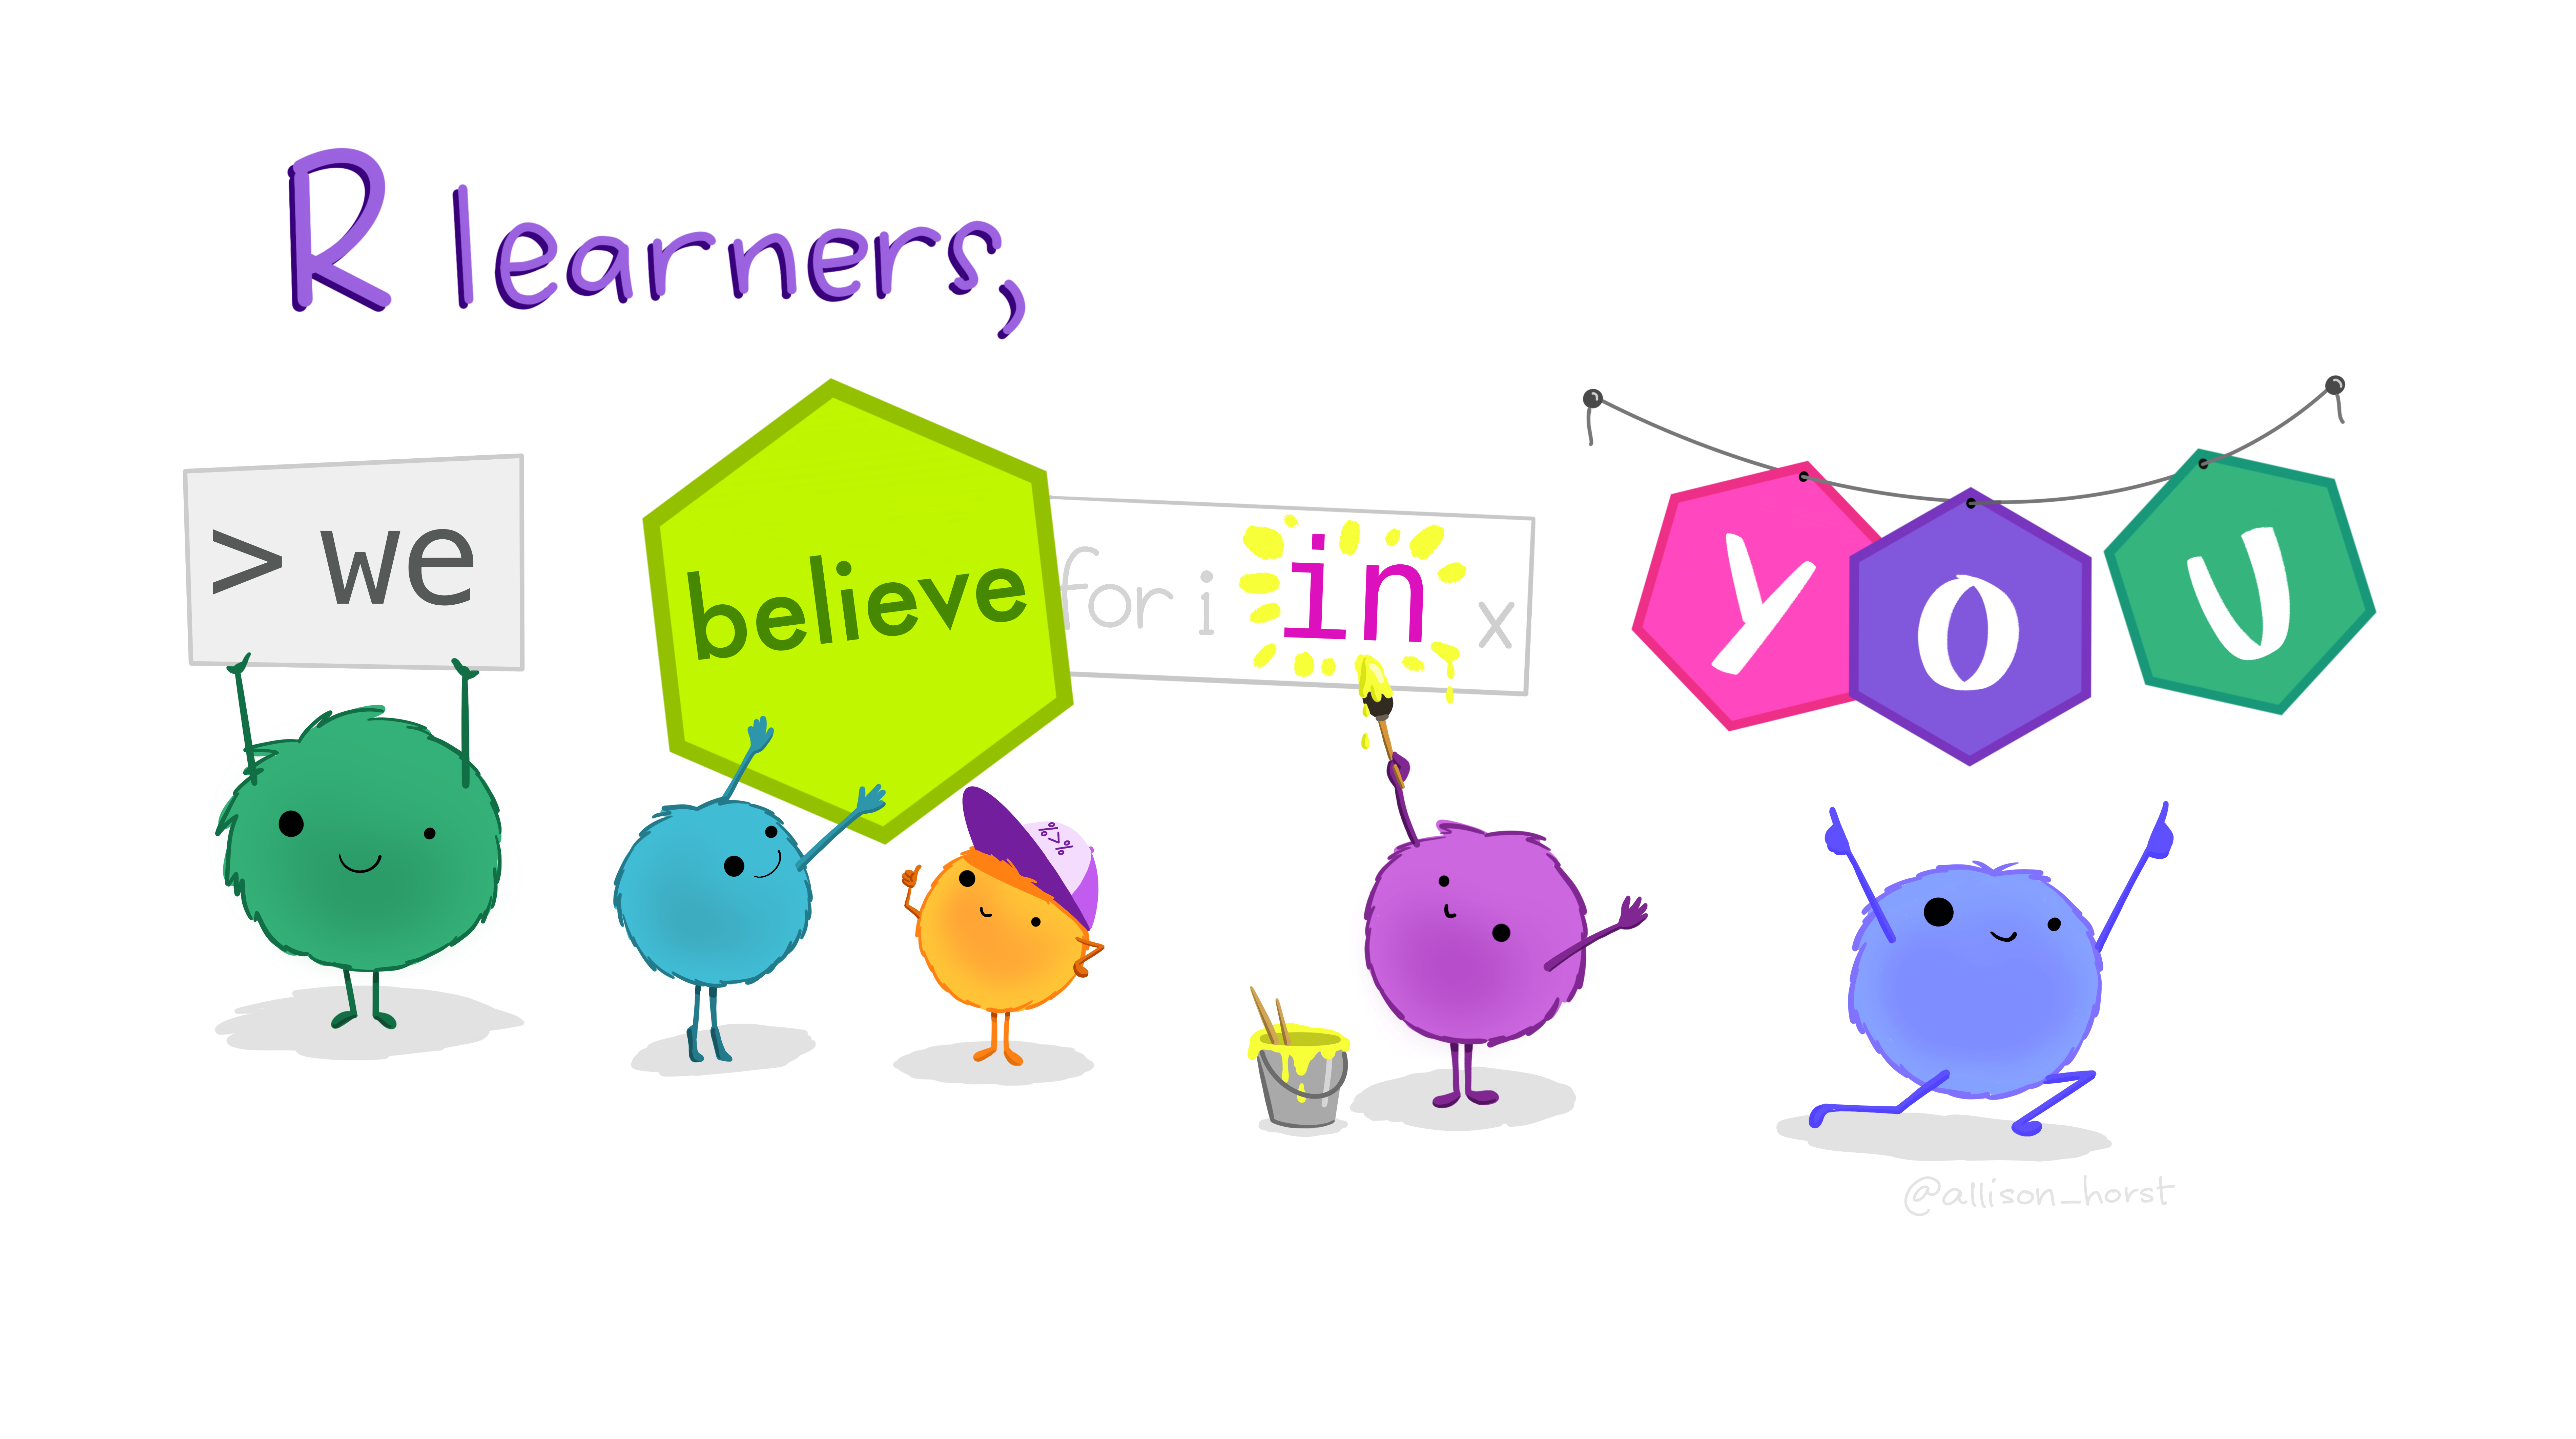
\includegraphics{images/RLearnersWeBelieve.png}

}

\caption{\emph{Artwork by @allison\_horst}}

\end{figure}%

\bookmarksetup{startatroot}

\chapter{Open Scholarship}\label{open-scholarship}

This book aims to provide a stepping stone for students and scholars of
traditionally less quantitative and computational disciplines (such as
some branches of linguistics and language education research) to gather
first (hopefully positive!) experiences with statistical and
computational approaches to working with empirical data\footnote{Emprical
  data is based on what is experienced or observed rather than on theory
  alone.}. The underlying belief is that these methods ought to be
accessible to all, regardless of their academic background or personal
circumstances. To this end, this book embraces the principles of Open
Scholarship.

Open Scholarship ``reflects the idea that knowledge of all kinds should
be openly shared, transparent, rigorous, reproducible, replicable,
accumulative, and inclusive (allowing for all knowledge systems)''
(Parsons et al. 2022). For this to be the case, teaching materials need
to shared openly and the tools and software taught in these resources
need to be freely accessible, too. In the following, we will briefly
consider the role of Open Educational Resources (OERs) and open-source
software in our pursuit of Open Scholarship.

\section{Open Source}\label{open-source}

In line with its aim to provide an accessible introduction to statistics
and data visualisation, this textbook relies exclusively on open-source
software and programming languages, foremost \texttt{LibreOffice\ Calc},
\texttt{R} and \texttt{RStudio}. Open source refers to software whose
source code is available under a license that grants anyone the rights
to study, modify, and distribute the software to anyone and for any
purpose. If we think of a software application as a cake, the source
code is like its recipe. It contains the list of ingredients and the
steps to bake the cake. Open source means that the recipe is publicly
available. You can access it, read it, and use it to bake the cake. You
can also modify it to add your own twist, such as adding a new
ingredient or making it vegan, and share it with others. In the context
of software, this allows many people to collaborate, make improvements,
and share their versions, resulting in better and more diverse software.

Using open-source software in this introductory textbook means that
anyone\footnote{Provided that they have access to the internet and a
  functioning personal computer.} can download, install and use the
required software at no cost. However, it is very important to note that
not all free software (\emph{freeware}) is open source. Let us
illustrate the difference by comparing different spreadsheet programmes
as, in the following chapter, we will begin exploring tabular data
structures in a spreadsheet programme.

The most most widely used spreadsheet programme to date is undoubtedly
\texttt{Microsoft\ Excel}. Excel is a commercial, proprietary
spreadsheet editor which forms part of the Microsoft 365 package. As
such, to use Excel on your personal computer, you need to buy a license
or be a member of an organisation (e.g., your university or company)
that pays for such a license. It is true that Microsoft now also offers
a free (functionally limited) web-based version of Excel, yet this still
does not make it open source. This is because Microsoft does not share
the source code of any Excel version, which means that, even if they are
giving away free cake, we do not have the recipe to bake the cake
ourselves should the company decide to start charging money for the cake
or to no longer distribute it at all! Similarly, you may be familiar
with a popular, web-based alternative to Excel: \texttt{Google\ Sheets}.
Whilst it is (currently) free to use, as the name suggests, Google
Sheets is owned by Google and is therefore not open source, either. By
contrast, \texttt{LibreOffice\ Calc} is a project of The Document
Foundation (TDF) that provides a popular, free, open-source office
productivity software suite comparable to Microsoft 365 called
\texttt{LibreOffice}. LibreOffice is developed collaboratively by very
many different people across the world who all do so on a volunteer
basis. The Document Foundation estimates that there are 200 million
active LibreOffice users worldwide, about 25\% of whom are thought to be
students (figures from 2018, see LibreOffice 2024). Its popularity is
likely due to the fact that it not only uses open formats (e.g.,
\texttt{.odt} and \texttt{.ods}), but can also open and save to a range
of popular formats including those used by Microsoft (e.g.,
\texttt{.docx} and \texttt{.xlsx}).

\begin{quote}
\section*{Quiz time!}\label{quiz-time}
\addcontentsline{toc}{section}{Quiz time!}

\markright{Quiz time!}

1) Which of these is an open-source alternative to Microsoft Word?

~

2) Which of these is an open-source alternative to Microsoft Powerpoint?

~

3) Not only can software be open source, programming languages can, too.
In fact, most modern programming languages are open source. In this
book, we will focus on the open-source programming language \texttt{R}.
Which of these is another open-source programming language?

~

4) There are also many open-source operating systems. Which of these is
an open-source alternative to the operating system Windows?

~
\end{quote}

\begin{tcolorbox}[enhanced jigsaw, colbacktitle=quarto-callout-caution-color!10!white, rightrule=.15mm, breakable, toprule=.15mm, toptitle=1mm, colframe=quarto-callout-caution-color-frame, bottomrule=.15mm, coltitle=black, opacityback=0, titlerule=0mm, opacitybacktitle=0.6, title=\textcolor{quarto-callout-caution-color}{\faFire}\hspace{0.5em}{Task 1}, left=2mm, arc=.35mm, leftrule=.75mm, bottomtitle=1mm, colback=white]

Your first task is to \textbf{download} and \textbf{install}
\textbf{LibreOffice} as we will use its spreadsheet editor,
\textbf{LibreOffice Calc}, in the next few chapters.

\begin{itemize}
\item
  LibreOffice is available for Windows, Mac and Linux. You can download
  it from here:
  \url{https://www.libreoffice.org/download/download-libreoffice/.}
\item
  You will find detailed installation instructions here:
  \href{https://www.libreoffice.org/get-help/install-howto/.You}{https://www.libreoffice.org/get-help/install-howto/.}
\item
  Detailed documentation is also available in many different languages:
  \url{https://documentation.libreoffice.org/en/english-documentation/}
\end{itemize}

\end{tcolorbox}

\section{Open Education}\label{open-education}

The web-based version of this textbook is published as an Open
Educational Resource (OER) under the Creative Commons license:
\href{https://creativecommons.org/licenses/by-nc-sa/4.0/}{\texttt{CC\ BY-NC-SA}}.
This means that it is free to read and use, as well as edit, remix, and
expand upon, provided that a) the original author and source is
mentioned (as indicated by
\href{https://creativecommons.org/licenses/by-nc-sa/4.0/}{\texttt{BY}}),
b) any derived version is not made into a commercial product
(\href{https://creativecommons.org/licenses/by-nc-sa/4.0/}{\texttt{NC}}
stands for non-commercial), and c) that any derived versions of this
textbook (e.g., a translated version or a version adapted for
historians) are also shared with this same license
(\href{https://creativecommons.org/licenses/by-nc-sa/4.0/}{\texttt{SA}}
stands for share alike).

In line with the principles of Open Education, all of the datasets that
we will work with in this textbook have been published in Open Access,
which means that we can freely use them to learn about statistics and
data visualisation using real datasets from published research studies
in applied linguistics and language education.

\begin{figure}[H]

{\centering 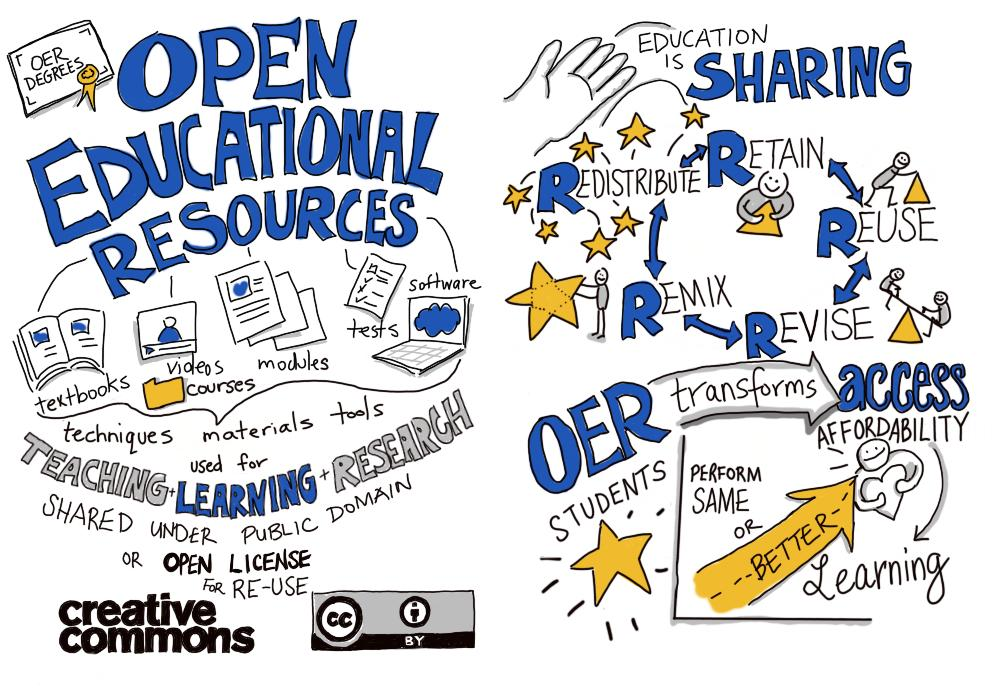
\includegraphics{images/oer.jpg}

}

\caption{OER sketch note by Yvonne Stry}

\end{figure}%

\begin{tcolorbox}[enhanced jigsaw, colbacktitle=quarto-callout-note-color!10!white, rightrule=.15mm, breakable, toprule=.15mm, toptitle=1mm, colframe=quarto-callout-note-color-frame, bottomrule=.15mm, coltitle=black, opacityback=0, titlerule=0mm, opacitybacktitle=0.6, title=\textcolor{quarto-callout-note-color}{\faInfo}\hspace{0.5em}{Tips to go further}, left=2mm, arc=.35mm, leftrule=.75mm, bottomtitle=1mm, colback=white]

This chapter has simplified things considerably. To be considered open
source, software distributions actually have to comply with ten
criteria. You can read up on them here:

\begin{itemize}
\tightlist
\item
  \url{https://opensource.org/osd}
\end{itemize}

To find out more about the benefits of open-source software in the
context of research, I recommend reading:

\begin{itemize}
\tightlist
\item
  \url{https://book.the-turing-way.org/reproducible-research/open/open-source}
\end{itemize}

To find out more about Open Educational Resources (OERs), I recommend
exploring the following OER databases:

\begin{itemize}
\item
  \url{https://oercommons.org/}
\item
  \url{https://www.twillo.de/oer/web/}
\end{itemize}

\end{tcolorbox}

\bookmarksetup{startatroot}

\chapter*{References}\label{references}
\addcontentsline{toc}{chapter}{References}

\markboth{References}{References}

\phantomsection\label{refs}
\begin{CSLReferences}{1}{0}
\bibitem[\citeproctext]{ref-LibreOffice2024}
2024. LibreOffice. \emph{Wikipedia}.
\url{https://en.wikipedia.org/w/index.php?title=LibreOffice&oldid=1218520104}.

\bibitem[\citeproctext]{ref-parsonsCommunitysourcedGlossaryOpen2022}
Parsons, Sam, Flávio Azevedo, Mahmoud M. Elsherif, Samuel Guay, Owen N.
Shahim, Gisela H. Govaart, Emma Norris, et al. 2022. A community-sourced
glossary of open scholarship terms. \emph{Nature Human Behaviour}.
Nature 6(3). 312--318. \url{https://doi.org/10.1038/s41562-021-01269-4}.

\end{CSLReferences}

\cleardoublepage
\phantomsection
\addcontentsline{toc}{part}{Appendices}
\appendix

\chapter{Next-step resources}\label{next-step-resources}

In the hope that this textbook has inspired you to dive deeper into the
wonderful world of quantitative data analysis, statistics, data
visualisation, and coding in R, here is a (work-in-progress) curated
list of further resources to continue your learning journey! \emph{Bon
voyage!} 🚀✨

\section{Recommended resources specific to the language
sciences}\label{recommended-resources-specific-to-the-language-sciences}

\begin{itemize}
\item
  Brezina, Vaclav. 2018. Statistics in Corpus Linguistics: A Practical
  Guide. Cambridge: Cambridge University Press.
  https://doi.org/10.1017/9781316410899.
\item
  Desagulier, Guillaume. 2017. Corpus Linguistics and Statistics with R:
  Introduction to Quantitative Methods in Linguistics (Quantitative
  Methods in the Humanities and Social Sciences). Cham: Springer
  International Publishing.
\item
  Gries, Stefan Thomas. 2013. Statistics for linguistics with R: a
  practical introduction. 2nd revised edition. Berlin: De Gruyter
  Mouton.
\item
  LADAL contributors. Tutorials of the Language Technology and Data
  Analysis Laboratory. \url{https://ladal.edu.au/tutorials.html}
  \texttt{Open\ Educational\ Resource}.
\item
  Levshina, Natalia. 2015. How to do linguistics with R: Data
  exploration and statistical analysis. Amsterdam: John Benjamins.
\item
  Schneider, Dr Gerold \& Max Lauber. 2020. Statistics for Linguists.
  \url{https://dlf.uzh.ch/openbooks/statisticsforlinguists/}
  \texttt{Open\ Educational\ Resource}.
\item
  Winter, Bodo. 2019. Statistics for Linguists: An Introduction Using R.
  New York: Routledge.
  \href{https://doi.org/10.1017/9781316410899}{https://doi.org/10.4324/9781315165547}.
\end{itemize}

\section{Further Open Educational Resources (in no particular
order)}\label{further-open-educational-resources-in-no-particular-order}

\begin{itemize}
\tightlist
\item
  Diez, David, Mine Cetinkaya-Rundel, Christopher Barr \& OpenIntro.
  2015. OpenIntro Statistics. Leanpub. \url{https://leanpub.next/os}.
\item
  Guide to Effect Sizes and Confidence Intervals:
  \url{https://matthewbjane.quarto.pub/guide-to-effect-sizes-and-confidence-intervals/}
\item
  Happy Git and GitHub for the useR: \url{https://happygitwithr.com/}
\item
  Quarto \& reproducibility:
  \url{https://ucsbcarpentry.github.io/Reproducible-Publications-with-RStudio-Quarto/index.html}
\item
  Modern Data Visualization with R:
  \url{https://rkabacoff.github.io/datavis}
\item
  Building reproducible analytical pipelines with R:
  \url{https://raps-with-r.dev/}
\item
  Modern Plain Text Computing:
  \url{https://mptc.io/content/01-content.html}
\item
  \url{https://www.data-to-viz.com/}
\item
  Interpreting data visualisation:
  \url{https://pressbooks.library.torontomu.ca/criticaldataliteracy/}
\item
  Improve your statistical inferences:
  \url{https://lakens.github.io/statistical_inferences/}
\item
  What they forgot to teach you about R: \url{https://rstats.wtf/}
\item
  Introduction to Data Science:
  \url{https://florian-huber.github.io/data_science_course/book/cover.html}
\item
  Data Science in Education Using R:
  \url{https://datascienceineducation.com/}
\item
  Models Demystified: A Practical Guide from t-tests to Deep Learning
  \url{https://m-clark.github.io/book-of-models/}
\item
  Data Visualization in R
  \url{https://datavizf23.classes.andrewheiss.com/}
\end{itemize}



\end{document}
